\section{Fast Convergence}

How to retrieve connectivity as fast as possible ($<$ 50 ms) after link / node failure?

\subsection{Overview}

\paragraph{Network / Routing Convergence}
A transition from a routing and forwarding state to another state typically triggered by a change in the topology (sudden in case of failure, planned / controlled in case of maintenance like hardware / firmware updates or config changes).

Convergence is a distributed process during which routers might have an inconsistent view of the network - this can lead to traffic loss or unnecessary depletion of resources (forward traffic to a blackhole or into a forwarding loop).

\paragraph{Sources of Delay}
Four steps: local detection of a failure, communication of the failure, recomputation and update of the forwarding state. First three steps are in the order of milliseconds. Last step in the order of number of prefixes that need to be updated which can be very slow (hundreds of seconds).


\subsection{IP Networks}


\subsubsection{Fast Detection}

Fast node / link failure detection with high accuracy and low overhead.

\paragraph{Physical- / Link-Layer Signals}
Some physical- / link-layers, such as optical layers, can detect failures through the loss of light or carrier signal (e.g. Synchronous Optical Networking - SONET, Synchronous Digital Hierarchy - SDH, Dense Wavelength Division Multiplexing - DWDM).

This is often as fast as possible (few ms) and has virtually no overhead. Cons: only works for some types of physical- / link-layers (e.g. not available on Ethernet) and does not detect certain kinds of failure (e.g. link between a router and switch fails but for other router connected to switch it seems like connection is still up - even tho router communication is broken).

%TODO: check out examples


\paragraph{Hello / Keepalive / Beacons}
Adjacent routers regularly exchange Hello messages and signal a failure whenever $k$ of those are missed in a row. By default, each routing protocol comes with such a mechanism and allows to configure: frequency (interval) and dead interval. Works on any router platform and detects a wider range of failures (since it actually tests the forwarding path), but it's slow and a huge overhead.

\paragraph{Bidirectional Forwarding Detection (BFD)}
Protocol-agnostic hello-based service running directly in the hardware (instead of relying on the numerous protocol-based mechanisms causing overhead). Since it is hardware-based (software is also possible), we can send frequent hellos without stressing the CPU (small hello and dead interval - 50ms and 150ms). Configure other protocols to not run their hello mechanisms anymore.

Session(s) established between two systems via three-way handshake that are explicitly configured (no discovery).

Fast detection, low overhead and high coverage (tests actual paths) - especially when run in hardware. Unfortunately, not all routers can run BFD in hardware (modern ones are more likely to have it).

\paragraph{Conclusions}
Use link-layer mechanism when available, complement with hardware-based mechanism and fallback on protocol-based ones as last resort.


\subsubsection{Fast Propagation}

Flooding of failure detection should happen immediately and flooded packets are sent with absolute priority over rest of traffic. Note that often, only parts of the network need to be informed of a failure for convergence.


\subsubsection{Fast Computation}

\paragraph{Shortest-Path-Based Protocols}
Like OSPF, IS-IS, etc. Not a huge problem anymore since computing an entire shortest-path tree in a huge network only takes a few ms nowadays and incremental shortest-path computation can help scale this process further (but most vendors don't even bother since first thing is so fast and incremental introduces complexity and possible bugs).

\paragraph{BGP}
Difficult since computation is done per-prefix and BGP routers often don't even know alternate paths and need to search for one (since only one route per prefix is advertised). There exist BGP extensions that allow for the advertisement of multiple routes for a prefix even if its not a chosen one (internal routers now need to carry many more route in their routing tables). Common tradeoff between scalability and speed.


%TODO BGP convergence lookup, example lec 9


\subsubsection{Fast Updates}

Updating the Forwarding Information Base (FIB) is typically the key bottleneck to overcome in the convergence process. Total update time = number of prefixes times average update time per prefix.

\paragraph{Cheap Trick}
Prioritize FIB updates according to how much traffic each prefix sees.

\paragraph{Long Term Solution}
Reorganize the FIB data structure (data plane) s.t. it allows for fast incremental updates. Pre-compute backup state, pre-load in reorganized FIB, activate pre-loaded backup state upon detecting a failure. IGP (Dijkstra-based protocols) - LFA and BGP - PIC.

\paragraph{Loop-Free Alternates (LFA)}
Neighbor that can carry your traffic impacted by the failure without it bouncing back to you (LFA does not use you to reach destination that you want to reach but can't). N is LFA for S to D if dist(N,D) $<$ dist(S,D) $+$ dist(S,N) (assumes symmetrical weights).

Depending on topology, a subset of the links / prefixes will be protectable by LFAs (e.g. triangles / meshes lead to high coverage vs. ring-based which suck). Coverage(per-link LFA) $\leq$ coverage(per-prefix LFA).

%TODO how to calculate LFA coverage?

\begin{figure}[h]
	\centering
	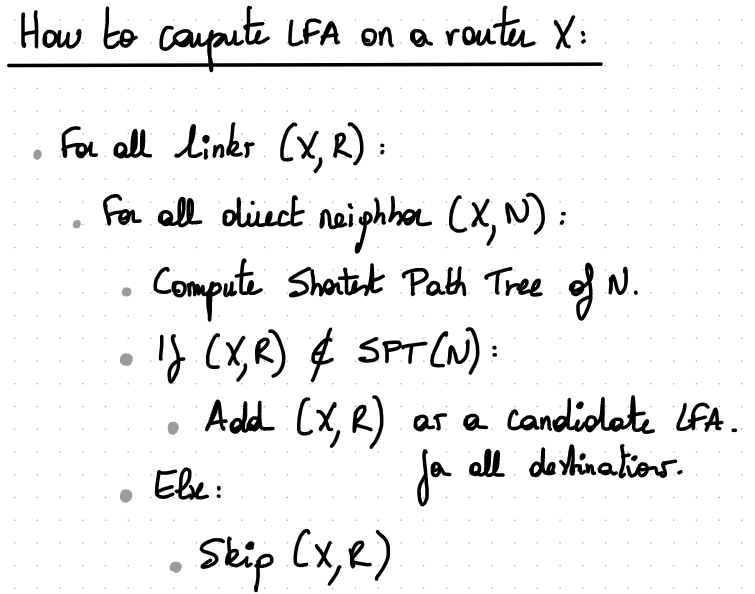
\includegraphics[scale=0.5]{images/4-lfa.PNG}
	\caption{Computing per-link LFAs for router X. Per-prefix LFAs can be calculated by evaluating each destination prefix instead each direct neighbor.}
	\label{fig:routing}
\end{figure}

%TODO examples lec 9

\textbf{Remote LFAs to increase coverage:} LFAs can be routers that are not directly connected by using tunneling (typically LDP-based). Does not guarantee full coverage!

\begin{figure}[h]
	\centering
	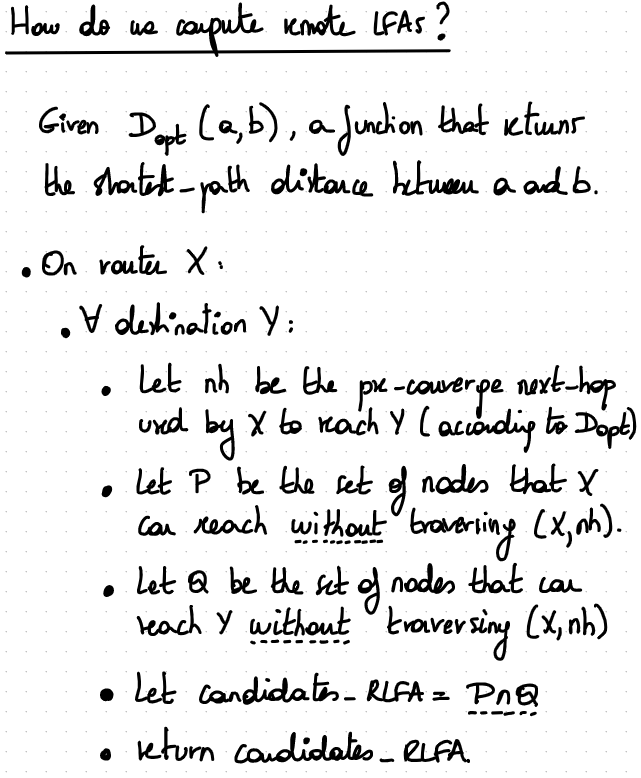
\includegraphics[scale=0.5]{images/4-remote.PNG}
	\caption{Computing remote LFAs.}
	\label{fig:remote}
\end{figure}

\textbf{FIB organization for fast activation:} one possible solution (which works well in P4) is to store two tables, one for mapping prefixes to a primary and a backup next-hop which are stored in the metadata of a packet and one for mapping each next-hop to a status (0 or 1) where if it's down (= 0) packet should use the backup next-hop.


\paragraph{Prefix-Independent Convergence (PIC)}
Enable the routers to quickly switch over to pre-installed alternate paths upon failures that affect BGP routes. The problem with standard BGP is "flat" FIBs where all reachable prefixes are mapped to a gateway routers egress interface.
%TODO ?????? google this


\subsection{MPLS Networks}

Easier than IP-based since we don't have distributed computations (as much).

Pre-establish secondary LSPs that don't carry any traffic to prepare for failures of important primary LSPs. Switching to the secondary LSP upon failure can be done immediately since there is no need for any coordination (provided the secondary LSP exists and is not impacted by the failure).

\subsubsection{End-To-End LSP Protection}

Ingress LSR establishes secondary LSP between ingress and egress LSR that relies on disjoint physical resources (router-disjoint and / or link-disjoint LSP) by using its path selection algo (signaled with RSVP-TE). Upon failure on primary LSP, adjacent router sends \textit{PathErr} message to ingress which triggers the switch to the secondary LSP.

Pro: ingress can immediately activiate secondary LSP without any coordination. Cons: one protection LSP must be established for each primary LSP, doubling the amount of memory needed. Failure info (\textit{PathErr}) must travel all the way to the ingress LSR before connectivity can be retrieved (slow!).


\subsubsection{Local LSP Protection}

Each LSR crossed by the primary LSP signals a protection LSP to cover for the failure of each link used by the primary LSP (can be generalized to router failures).

Pro: traffic can be immediately switches onto protection LSP by router detecting the failure (and not just by ingress). Con: depending on the network, a large number of protection LSPs might be required.

\begin{figure}[h]
	\centering
	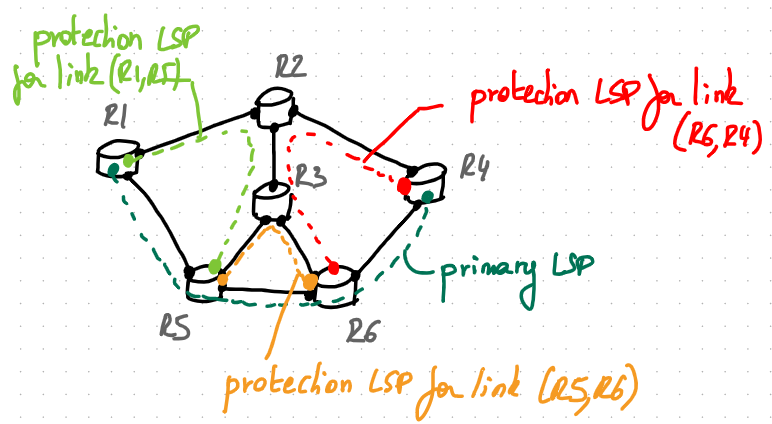
\includegraphics[scale=0.5]{images/4-local.PNG}
	\caption{Example for local LSP protection.}
	\label{fig:local}
\end{figure}